\section{Temporal Analyses}
\label{sec:results}

In this section I show different analysis to discover and characterize how the FFCS are used. In the first part of the section, I analyse the temporal systems characterization to understand if FFCS are actually used and when.

I consider a period from December 10th 2016 to January 31st 2017, the first reliable collected data chunk. The system observed 125,000 snapshots, about 104,000 bookings for car2go and 93,000 for Enjoy. In Turin, the fleet of car2go was composed by 394 cars, and the fleet of Enjoy was composed by 172 cars.

In order to make clear the rest of the book, it necessary to univocally define the basilar entities related to the car status in the data lake defined in the chapter \ref{chap:2_dataset}, section \ref{sec:2_4_data_normalization}.

\begin{definition}{the \textbf{Parking}}
	\label{def:parking} is the time period in which the car is present in, at least, two consecutive snapshot. Therefore that car it is available for an user reservation
\end{definition}
\begin{definition}{the \textbf{Booking}}
	\label{def:booking} is the time period in which the car is NOT present in, at least, two consecutive snapshot. There fore an user booked that vehicle or the provider temporary removed it for maintenance.
\end{definition}


\subsection{System Utilization}

\begin{figure}
\centering
 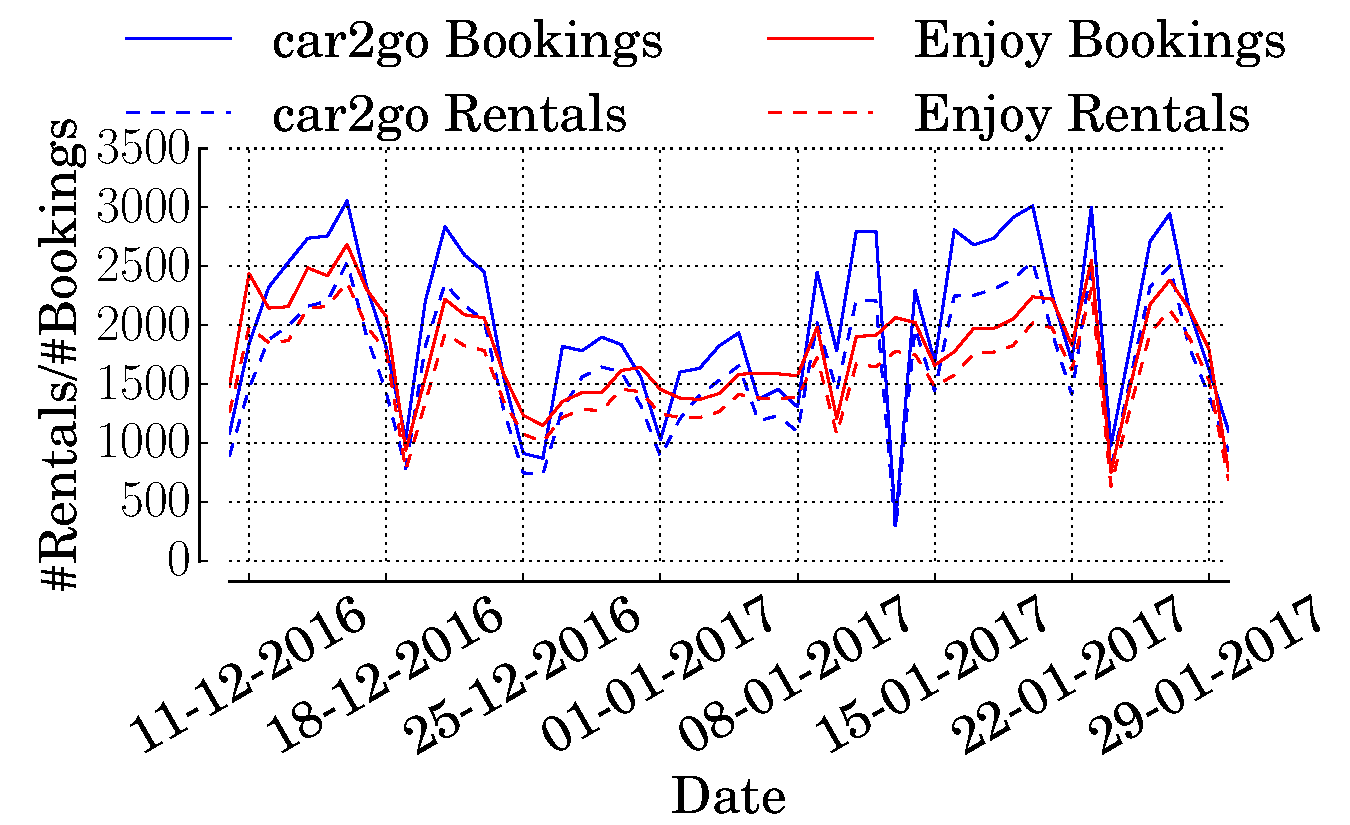
\includegraphics[width=0.85\columnwidth]{figures/bookings.pdf}
 \caption{Total number of bookings and of rentals per day for car2go and for Enjoy \label{fig:bookings}}
\end{figure}
The providers, in this case study, allows the users to \textit{reserve} a car before the ride. More in details, the provider makes the reserved car unavailable for the other users without billing the customer who reserved the car. When the reservation time (that changes for each provider), the billing mechanism starts even if the engine it is still off. The customer can cancel the reservation without any expense if it happens before the reservation time. With this mechanism, the providers would let the possibility to the users to reach the cars by foot.

Given that, it is now possible to the define:
\begin{definition}{\textbf{Reservation}}
	\label{def:reservation} A reservation it is a booking where the initial and final destination matches and the duration is lower than the provider's reservation time.
\end{definition}

\begin{definition}{\textbf{Rental}}
	\label{def:rental} A rental it is a booking where the initial and final destination are different.
\end{definition}


Starting from December 10th, Figure~\ref{fig:bookings} plots the total number of bookings and the total number of rentals recorded on each day, for car2go (blue curves), and for Enjoy (red curves). Obviously, being the latter a subset of the first, its number is always smaller. However, during some days, the discrepancy is well visible; that means that the operation of booking cancellation is not so rare.

Interestingly, firstly, both car2go and Enjoy follow a similar behaviour with the number of bookings and rentals decreasing in the Christmas period and increasing again after the Epiphany. 

Secondly, despite car2go fleet has more than twice as much cars than Enjoy (394 vs. 172), the number of car2go bookings does not show such a higher value with respect to Enjoy. With Enjoy having more bookings in some snapshots e.g., December 10th and 11th. Moreover, in some points (ecember 19th, January 24th) it is possible to detect huge drop due to the failure of our crawler. 

Moreover, some drops in bookings' values are noticeable. Those sudden changes can be addressed to some failures, in the crawlers (e.g., when all curves suddenly drop) or in the operators' web services(e.g., when only one system suffers a sudden drop).



\begin{figure}
\centering
 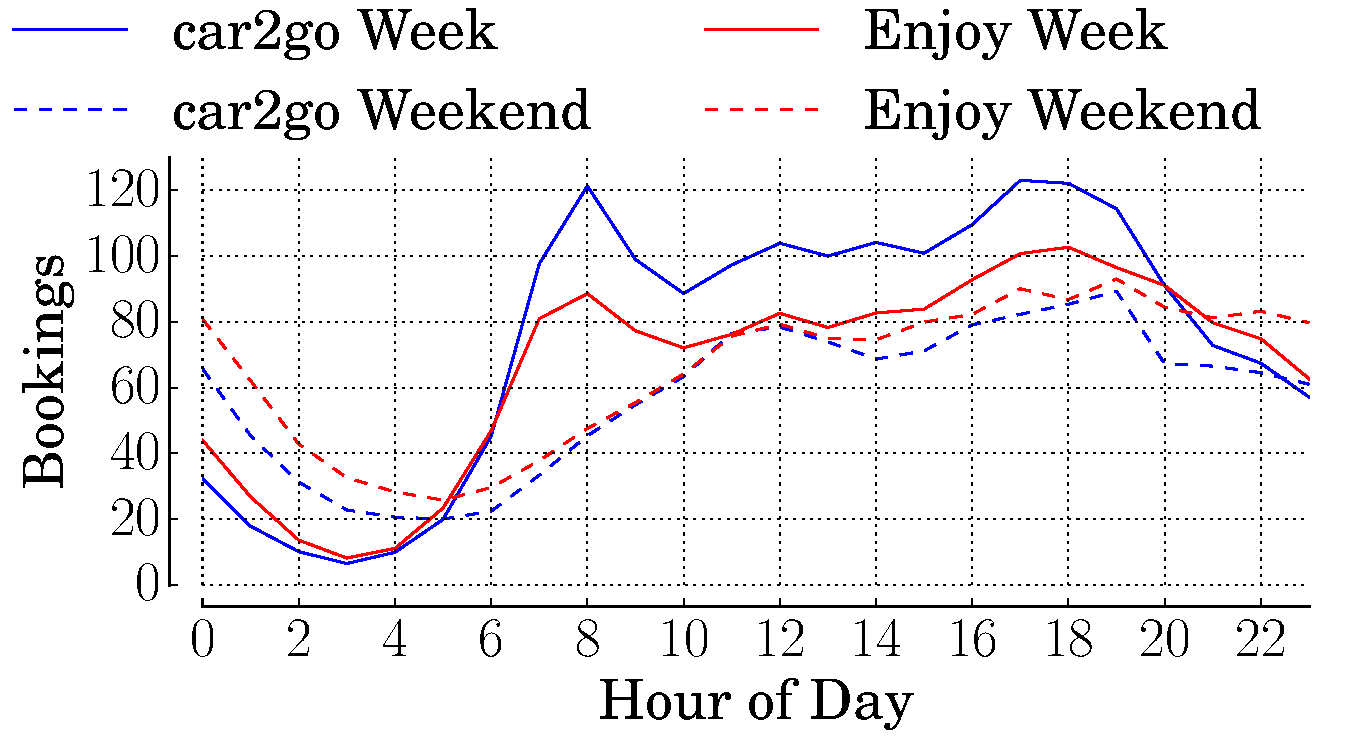
\includegraphics[width=0.85\columnwidth]{figures/bookings_day.pdf}
 \caption{Mean number of bookings in weekdays and weekends for car2go and Enjoy\label{fig:bookingsweek}}
\end{figure}

Looking at the data with a finer granularity, it is noticeable that the car sharing adoption changes during the day. To better characterize this, I separate weekdays and weekends. The figure~\ref{fig:bookingsweek} points out the trend over the day. The curves report the average number of bookings over the entire period  in each hour of the day.

Firstly, it is possible to see that weekdays and weekends have a quite different trend. During the weekend FFCS systems are more used at night with respect than weekdays, with on average at midnight of 80 and 60 bookings per hour for Enjoy and car2go. Instead, the figure shows how during the weekdays both car2go and Enjoy have their peak of usage at 8~am and between 5~pm and 7~pm. This trend can be easily explained as, during that time slots, FFCS customers use cars to go and return from work. 
As previously indicated, despite car2go has twice the number of cars than Enjoy, the system utilization of the latter is higher, with peak utilization topping to 60\%, versus 30\% of car2go. 

Even in absolute number of rentals, Enjoy shows an higher number of bookings after 8~pm during the weekdays, and always during the weekends. This can be explained by the car models adopted by the two companies. While car2go uses the compact-two seats \textit{Smart}, Enjoy fleet is composed of \textit{Fiat 500}, which are 4 seats cars. Rentals prices are instead comparable (0.24\euro/min Enjoy vs 0.25\euro/min car2go). Data suggests that Enjoy looks more appealing during the times when people prefer to share the ride, and during weekends when families and groups move. 



\section{Rides Characterization}
In this section, I give a detailed look about driving habits. In particular I compare driving distances and duration of rentals and parking duration. Finally I conclude with some insights about the variation of spatial demand, characterizing which and because some zones attract or generate more rentals with compared to other one.


\subsection{Driving patterns}


%\begin{figure}[t!]
%	\centering     %%% not \center
%	\subfloat[][ECDF of the booking duration when the booking does not produce a rental. Weekdays and weekends]
%	{\label{fig:3_5_pdf_norent}
%		\includegraphics[width=0.33\columnwidth]
%		{figures/no_rent.pdf}
%	}
%	\subfloat[][ECDF of the rental duration. Weekdays and weekends]{\label{fig:3_5_cdf_duration}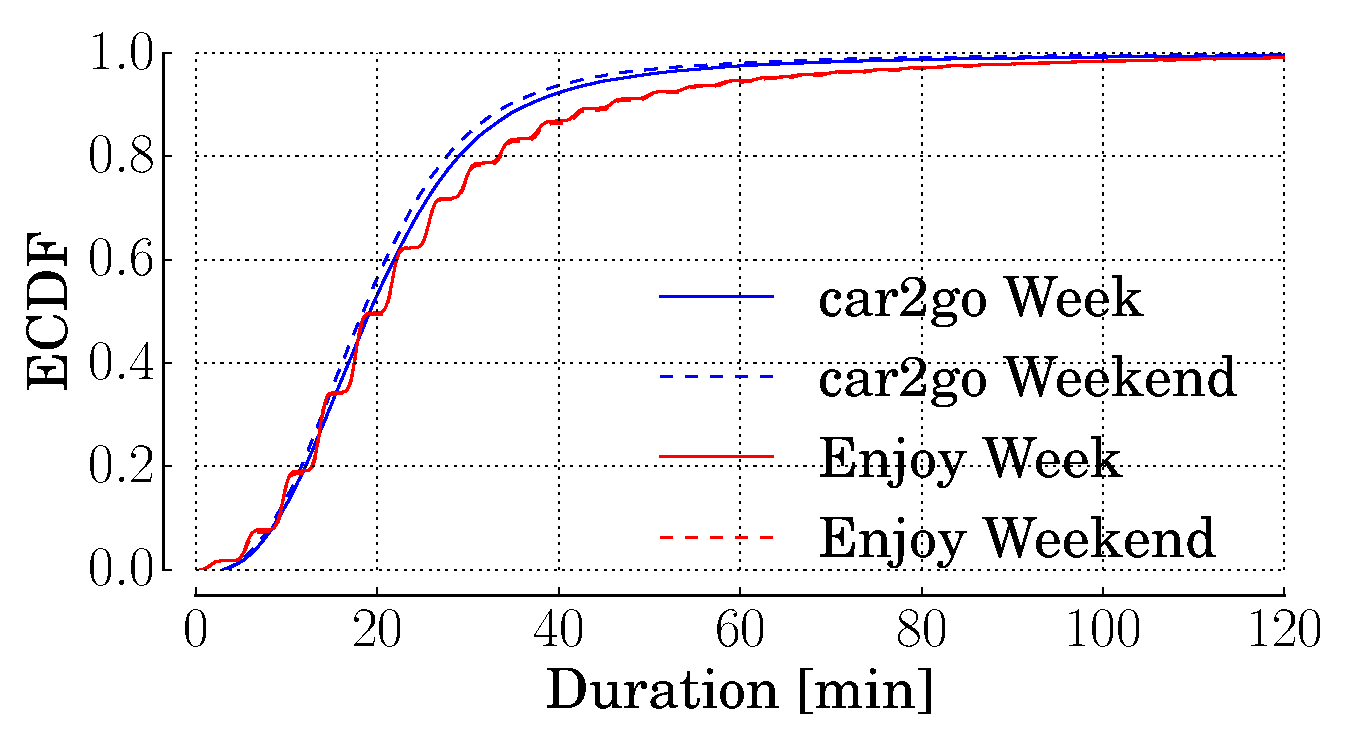
\includegraphics[width=0.33\columnwidth]{figures/duration.pdf}}
%	\subfloat[][ECDF of the rental distance. Weekdays and weekends]{\label{fig:3_5_cdf_distance}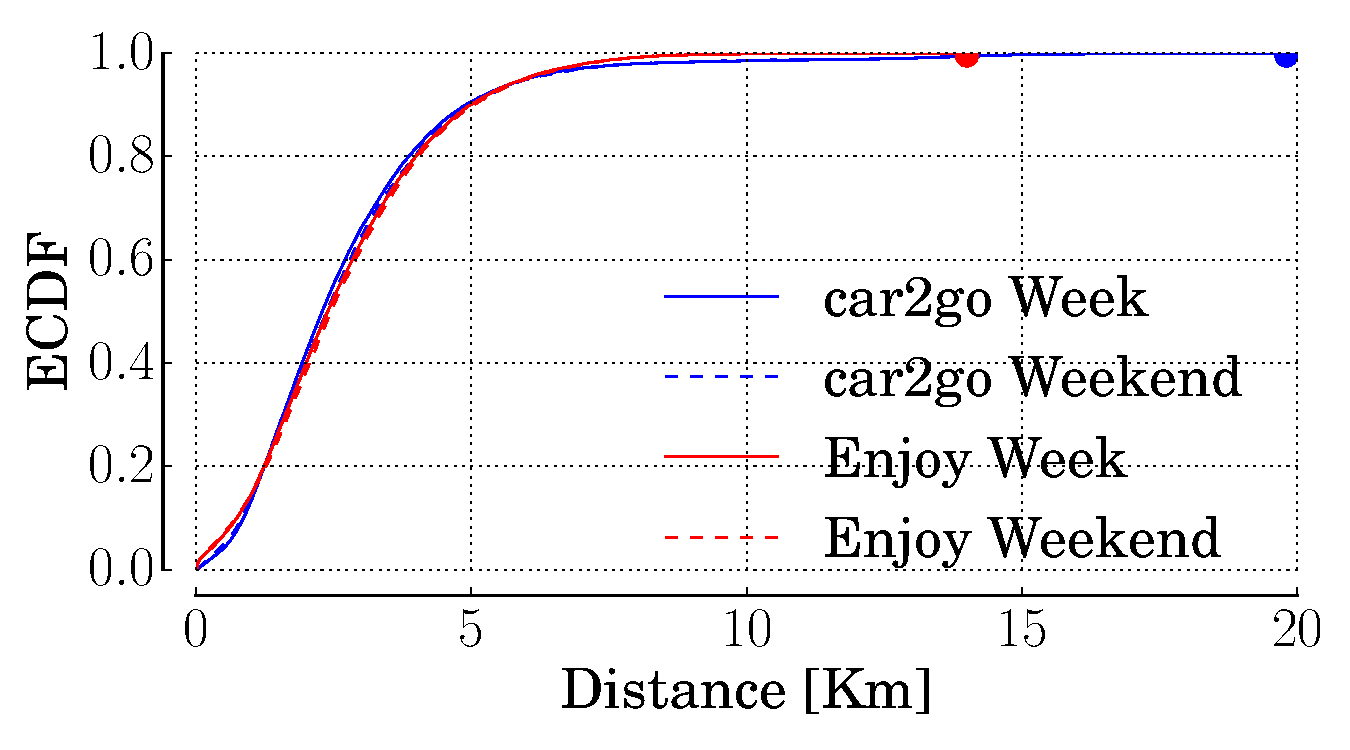
\includegraphics[width=0.33\columnwidth]{figures/distance.pdf}}
%	\caption{Users' booking and rentals habits \mc{magari immagini singole}}
%	\vspace{-3pt}
%\end{figure}


Now, I show how users tend to use FFCS systems during weekdays and weekends. I study three different aspects of users' behaviour: 
\begin{itemize}
	\item for how long users reserve the car before cancelling a booking (Figure~\ref{fig:3_5_pdf_norent})
	\item for how long users rent a car (Figure~\ref{fig:3_5_cdf_duration})
	\item how far users drive (Figure~\ref{fig:3_5_cdf_distance})
\end{itemize}

\begin{figure}
	\centering
	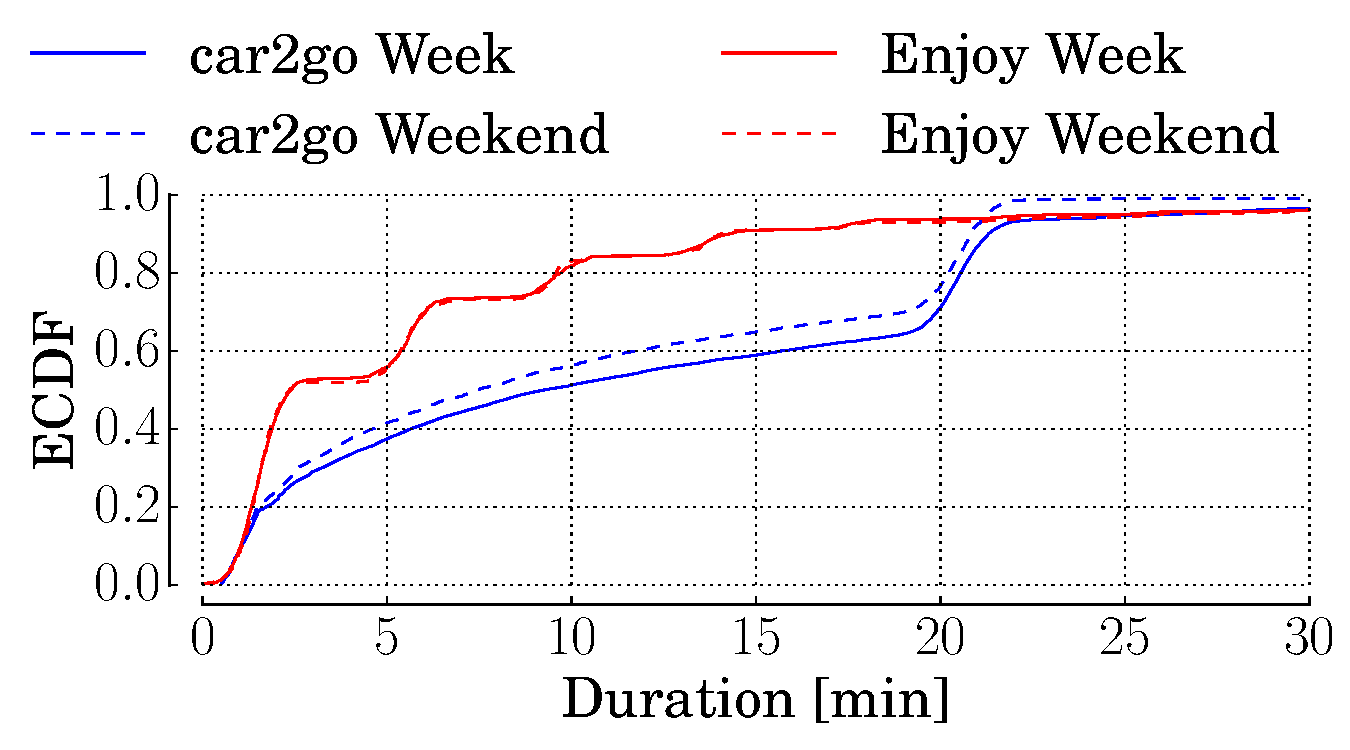
\includegraphics[width=0.85\columnwidth]{figures/no_rent.pdf}
	\caption{ECDF of the booking duration when the booking does not produce a rental. Weekdays and weekends \label{fig:3_5_pdf_norent}}
\end{figure}

First, I check if and for how long users reserve a car and then they cancel a booking. Interestingly, only a small subset of Enjoy bookings are affected by cancellation with respect to car2go bookings. In particular, the dataset presents 14.9\% of car2go and 2.9\% of Enjoy bookings cancellation. This again hints for people preferring to use the Fiat 500 offered by Enjoy, so that they hardly cancel a booking when they reserved an available vehicle. On the contrary car2go availability is higher and so it looks easier to find a closer car. People may thus cancel a previous booking when they find a closer vehicle. Another hypothesis is that car2go may be used as a ``backup'' until an Enjoy vehicle becomes free in the user's area. 

Looking at when people cancel the reservation, figure~\ref{fig:3_5_pdf_norent} shows the CDF of reservation time. Indeed, car2go tends to have a smaller percentage of cancellation within 5 minutes, with a huge step at about 20 minutes. While the first ramp can be explained as a communication error or as some sudden cancellation, the latter can be explained by the \textit{maximum free-of-charge reservation time} of car2go. Truly, users, may reserve a car up to 20 minutes without paying any fee. The same trend is not present for Enjoy which offers a \textit{maximum free-of-charge reservation time} of 15 minutes. Instead, the curve shows a peak at 2 minutes and then a decreasing trend after 15 minutes, when almost all the cancellation are already done.
One last important aspect that this picture shows is how the Enjoy curves have some steps instead of being smooth as the car2go ones. 
This hints to periodic updates on web system so that a time granularity emerges.
To shed some lights on this phenomenon, I performed some active experiments with the Enjoy web portal. The experiment consists of making a new reservation and find when our crawler detects that the car actually disappears from the set of available cars. Then, as soon as I spot the car disappearing, I cancel the reservation to detect when the car reappears in the system. Surprisingly, I discover that when we make the reservation, the car immediately disappears from the system, instead, when I cancel the reservation, the system takes between 1 and 4 minutes to actually show the car again. The presence of such an offset causes the steps in the Enjoy curves which are affected by an artificial delay. To take into account this offset all Enjoy duration have been decreased of 2.5 minutes, i.e., the average delay the Enjoy system adds. 


\begin{figure}
	\centering
	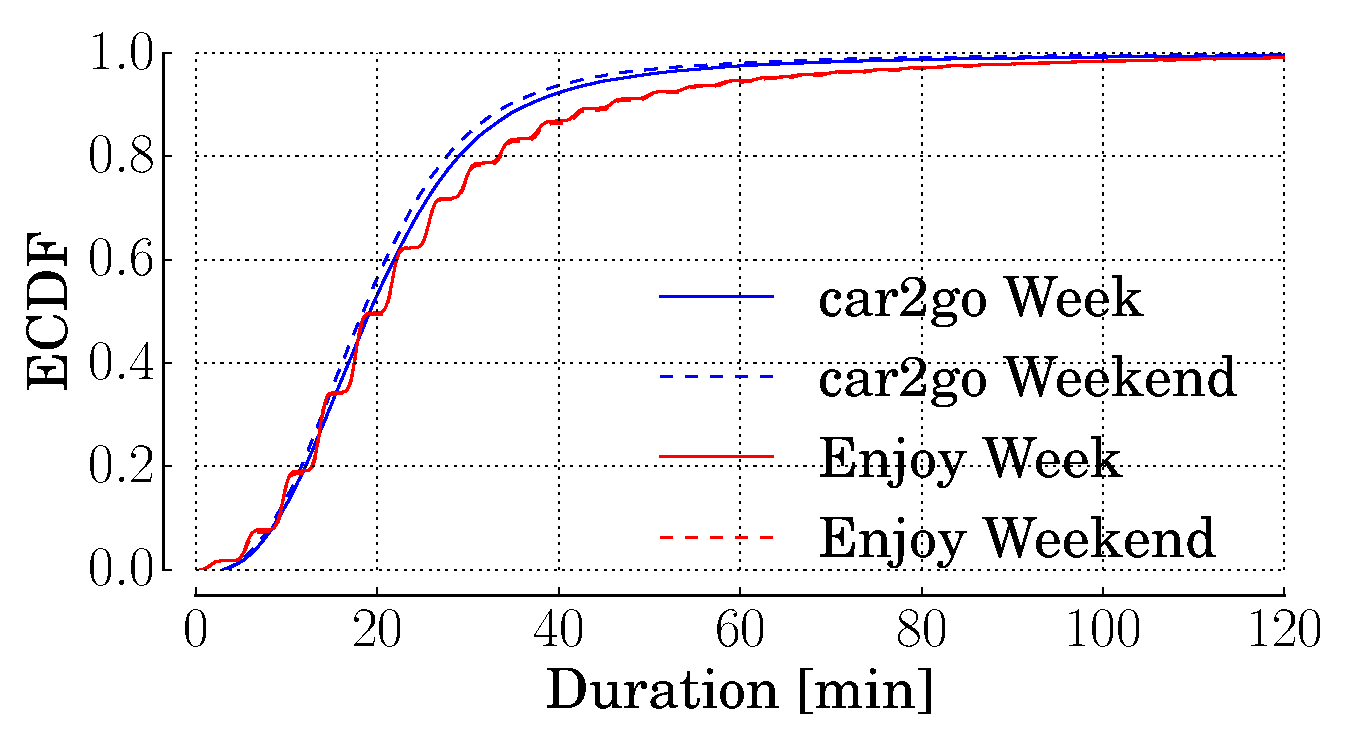
\includegraphics[width=0.85\columnwidth]{figures/duration.pdf}
	\caption{ECDF of the rental duration. Weekdays and weekends\label{fig:3_5_cdf_duration}}
\end{figure}


I next move to characterize the rental duration. Figure~\ref{fig:3_5_cdf_duration} depicts the Empirical Cumulative Distribution Function (ECDF) of the booking duration for Enjoy and car2go during the weekdays and the weekends. The plot shows how the trend tends to be equal during the weekdays and the weekends. This demonstrates that, despite the different pattern of utilization shown before, the booking duration time results similar. Secondly, the ECDFs of car2go and Enjoy are almost overlapped, highlighting how these two services tend to be used in a similar way. Indeed, most of the rentals last less than 1 hour, with 80\% of them lasting less then 30 minutes. It is important to remark that this times include also the reservation time, i.e., the time the user can reserve a car for free before driving it, and the time to find a parking place. Therefore the actual driving time may be significantly smaller.


\begin{figure}
	\centering
	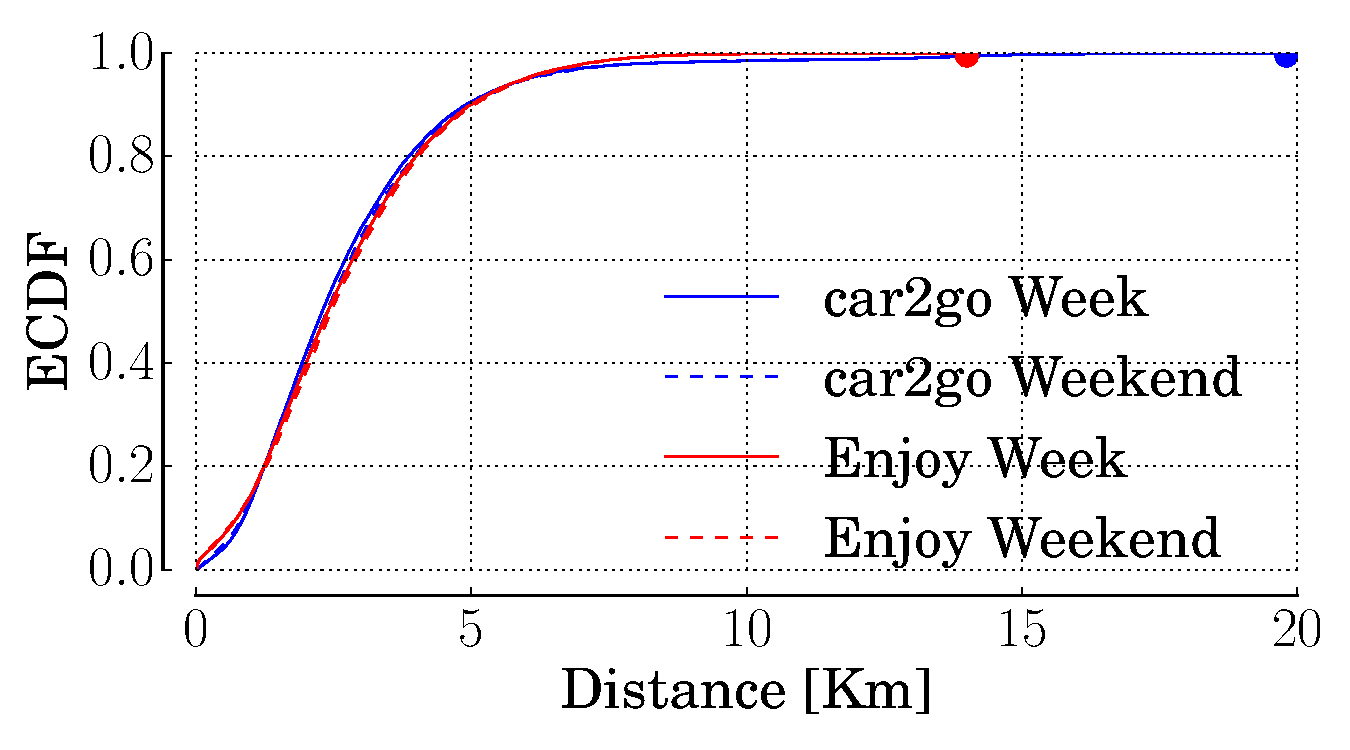
\includegraphics[width=0.85\columnwidth]{figures/distance.pdf}
	\caption{ECDF of the rental driven distance. Weekdays and weekends\label{fig:3_5_cdf_distance}}
\end{figure}


I repeat the same analysis considering the driving distance as reported in Figure~\ref{fig:3_5_cdf_distance}.
To determine the driving distance of each trip we exploit the Google Direction APIs to get the shortest path from the origin to the destination. Similarly, for the driving duration, car2go and Enjoy show a comparable behaviour, and marginal changes during weekdays and weekends. Interestingly, the graphs points out that the 90\% of the trips last less then 5~km demonstrating that most of the rentals are used for short trips both in term of time, and in term of distance. Lastly, the car2go curves saturate many km later than the Enjoy ones as highlighted by the circles. This is due to the possibility to reach the airport of Turin with the car2go cars, which is about 20 km far. 



\begin{figure}[t!]
\centering
\vspace{-10pt}
 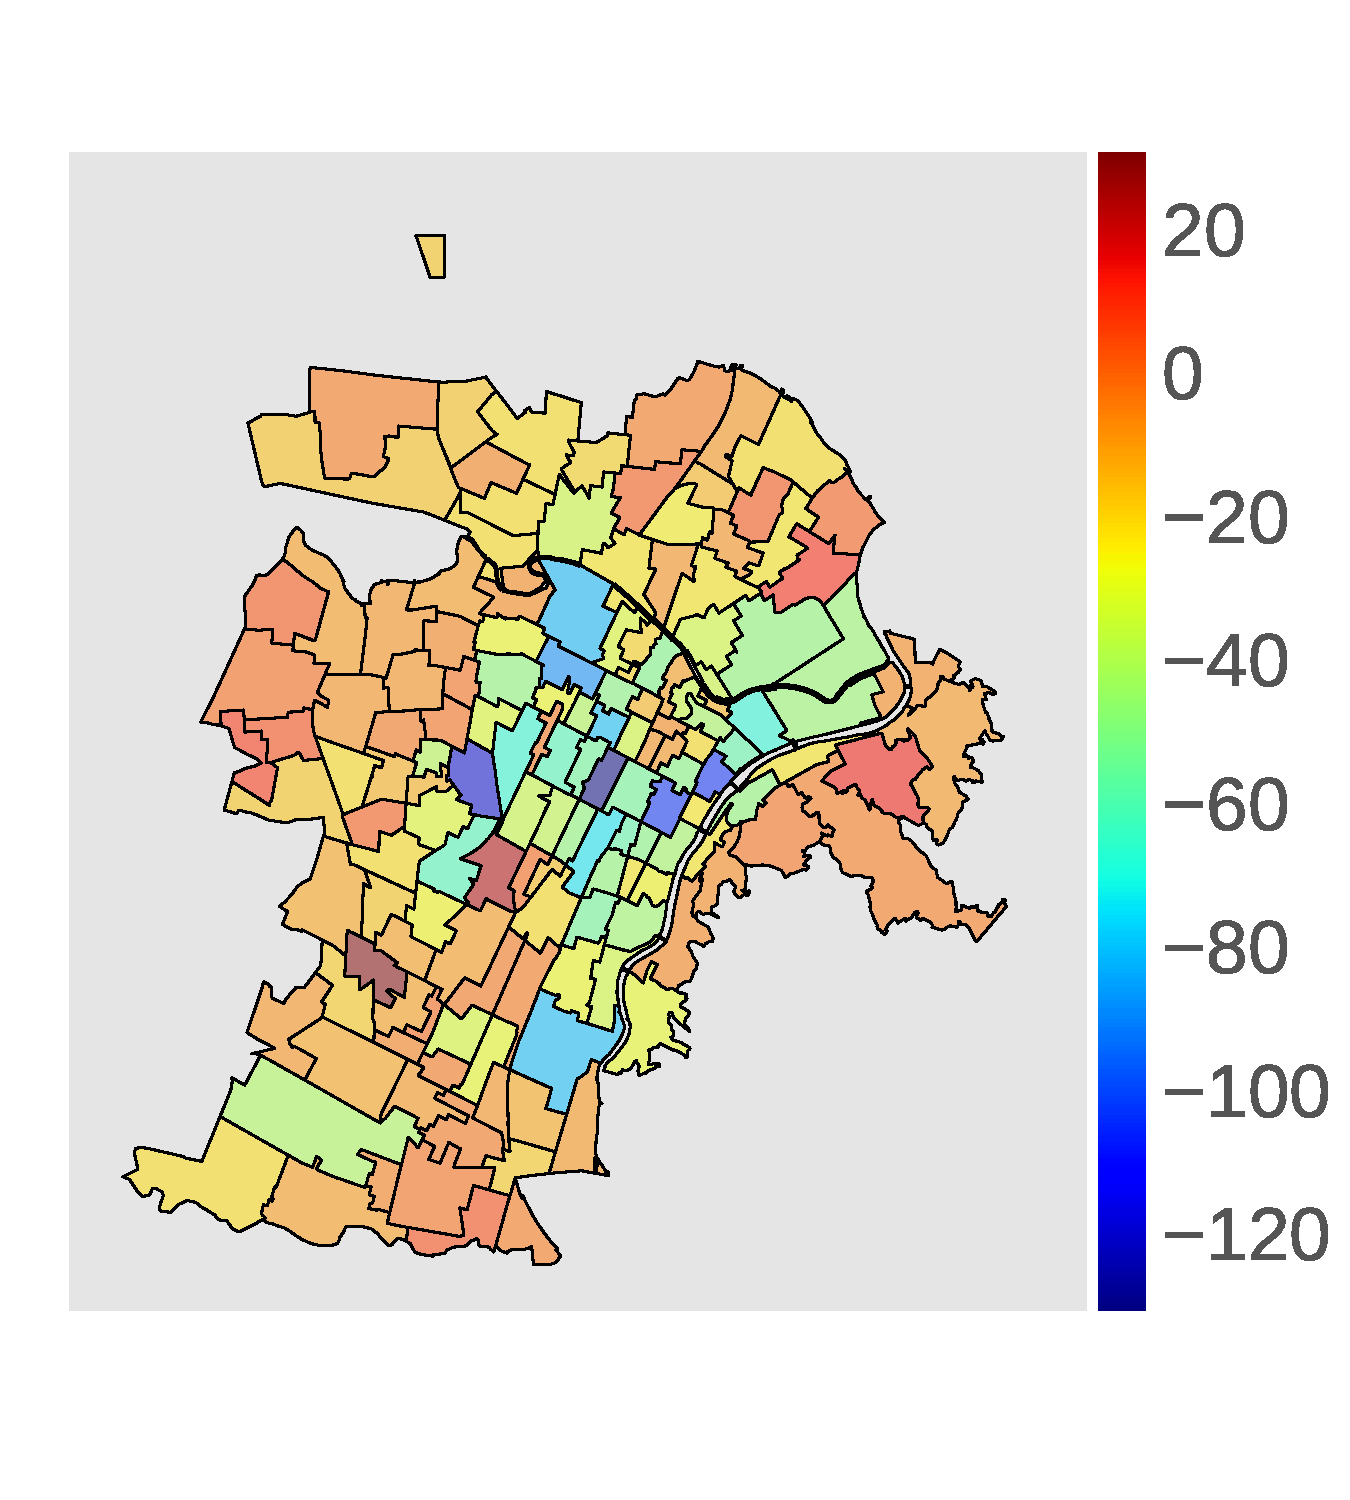
\includegraphics[width=0.72\columnwidth]{figures/clorophlet_o_minus_o1.pdf}
 \vspace{-10pt}
 \caption{Heatmap of arrival - departure per area from 7~am to 12~am vs from 5~pm to 9~pm \label{fig:3_5_heatmap_arr_dep}}
\end{figure}


\subsection{Spatial Analysis}  


In the previous section I analysed car2go and Enjoy only from a temporal point of view. In order to have a complete scenario, it is necessary to study recurrent spatial patterns. To do that I projected the initial and final coordinates on the Turin's neighbour map. Then I computed the attractiveness of each neighbour. Figure~\ref{fig:3_5_heatmap_arr_dep} shows the attractiveness of the  zones in Turin by analyzing the departure and arrival zones. For each zone I compute the difference between bookings ended in the evening [5~pm - 9~pm] and bookings ended in the morning [7~am, 12~am]. Red {areas are those} more attractive during the evening, while blue areas are more attractive in the morning. It is clear that the city center is the most popular destination for car sharing during the office hours, while the trips are sparsely ending in the suburbs during the evening.


\subsection{Users' Habits}

I now characterize how users drive and what is the correlation between public transport usage and availability.

To observe users' driving habits, I use the \textit{driving time} returned by the Google Directions APIs to {obtain} the estimated {driving} time from {rental initial position to the rental final position}. Intuitively, the {rental} time is longer than the driving time as it takes into account also the {reservation} time, and the time to find a final parking spot. Figure~\ref{fig:3_5_heatmap_driving} shows an heat map where the X axis represents the Google estimated driving time and the Y axis the actual booking time. Each cell counts the number of {observed} trips {for each (x,y) pairs}.
For the ease of representation the values are rounded by minute. The diagonal line separates the area where the booking time is lower/greater than the driving time. As expected, most of the trip falls in the area where the booking time is greater then the driving time. However, a non negligible number of trips (12.1\%) falls in the area where the booking time lasts less than the driving time. 

\begin{figure}[h!]
	\centering
	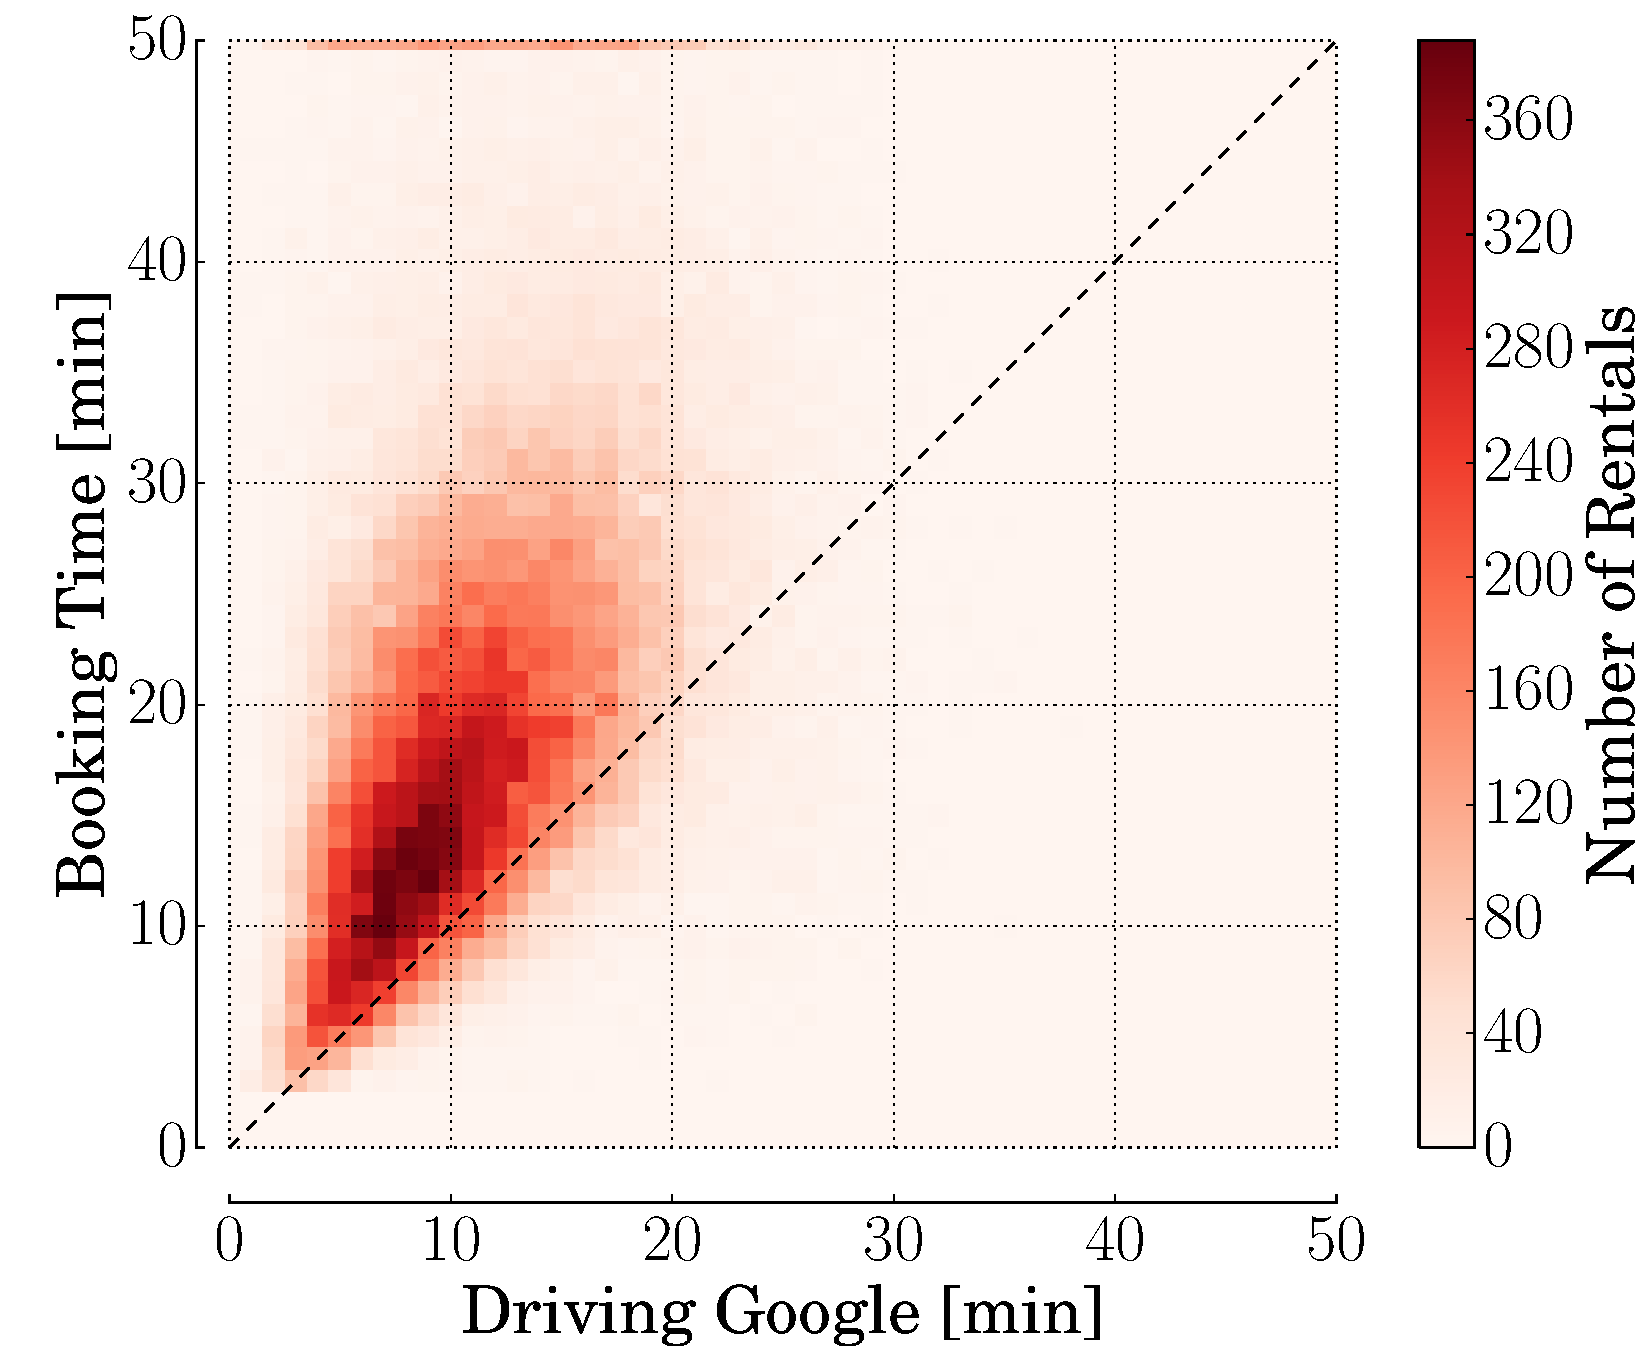
\includegraphics[width=0.85\columnwidth]{figures/car2go_faster_driving.pdf}
	\caption{Heatmap of booking time vs estimated driving time by Google\label{fig:3_5_heatmap_driving}}
\end{figure}


This may be due to several factors: Google Directions possibly overestimating the average trip duration, or users driving faster than expected.
To better quantify how much faster users drive the car in those cases, I  computed the difference between the driving time and the actual booking time. I show the Empirical Cumulative Distribution Function of such values in Figure~\ref{fig:3_5_cdf_faster_google}. It is possible to see that te most of these trips are only 5 minutes faster than the estimated driving time, with Enjoy users which seems to drive faster than car2go ones. Indeed, if the trip is more than 10 minutes faster, Google suggested a longer path to the destination, e.g., suggesting to take the highway which was much longer with respect to crossing part of the city.

This analysis hints that the current pricing policy, which depends only by the booking time, may have some drawbacks as it may encourage users to drive fast. An hybrid pricing policy, which takes into account both the time and the distance, may be effective in solving this problem, e.g., by increasing the price in case of an user drive faster than expected, or by reducing the fee in case of traffic congestion.

\begin{figure}[h!]
	\centering
	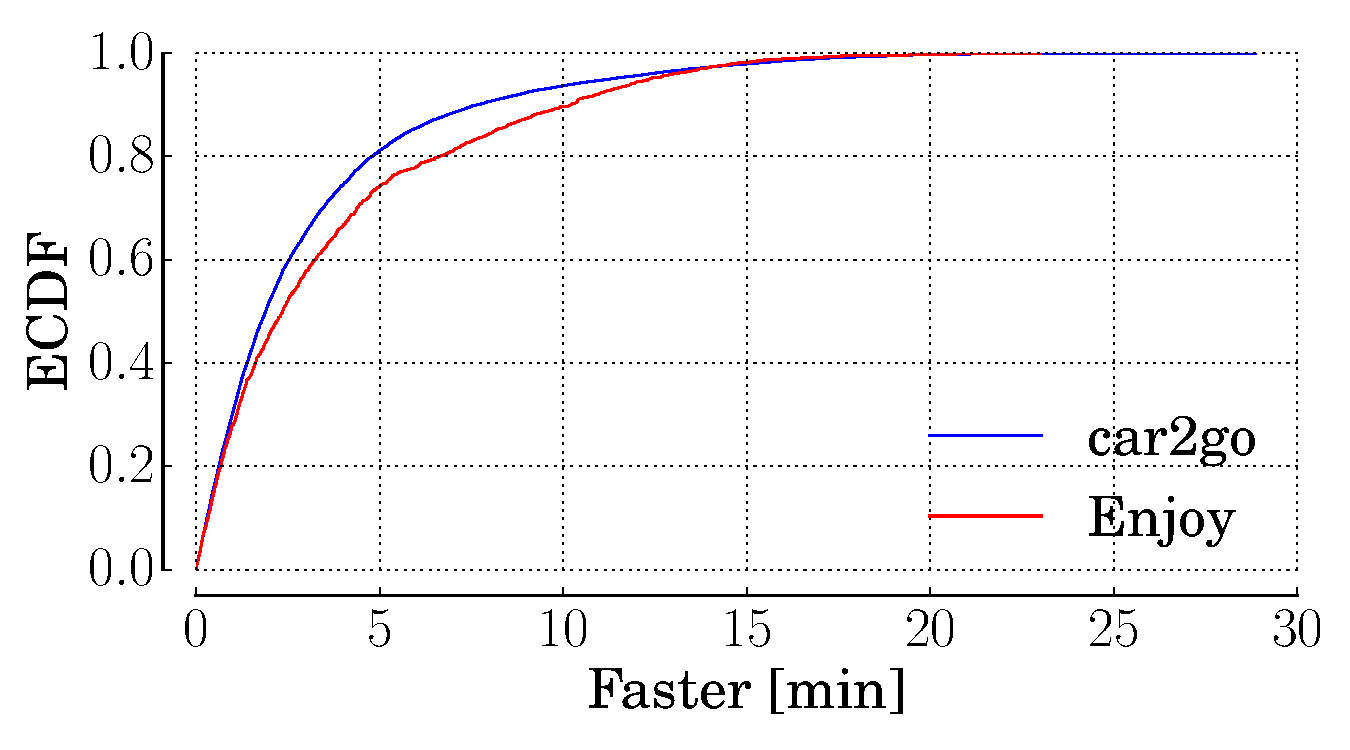
\includegraphics[width=0.85\columnwidth]{figures/faster_driving.pdf}
	\caption{ECDF of the difference between the expected driving time and the actual driving time\label{fig:3_5_cdf_faster_google}}
\end{figure}


%\begin{figure}[t!]
%\centering     %%% not \center
%\subfloat[][Heatmap of booking time vs estimated driving time by Google]{\label{fig:heatmap_driving}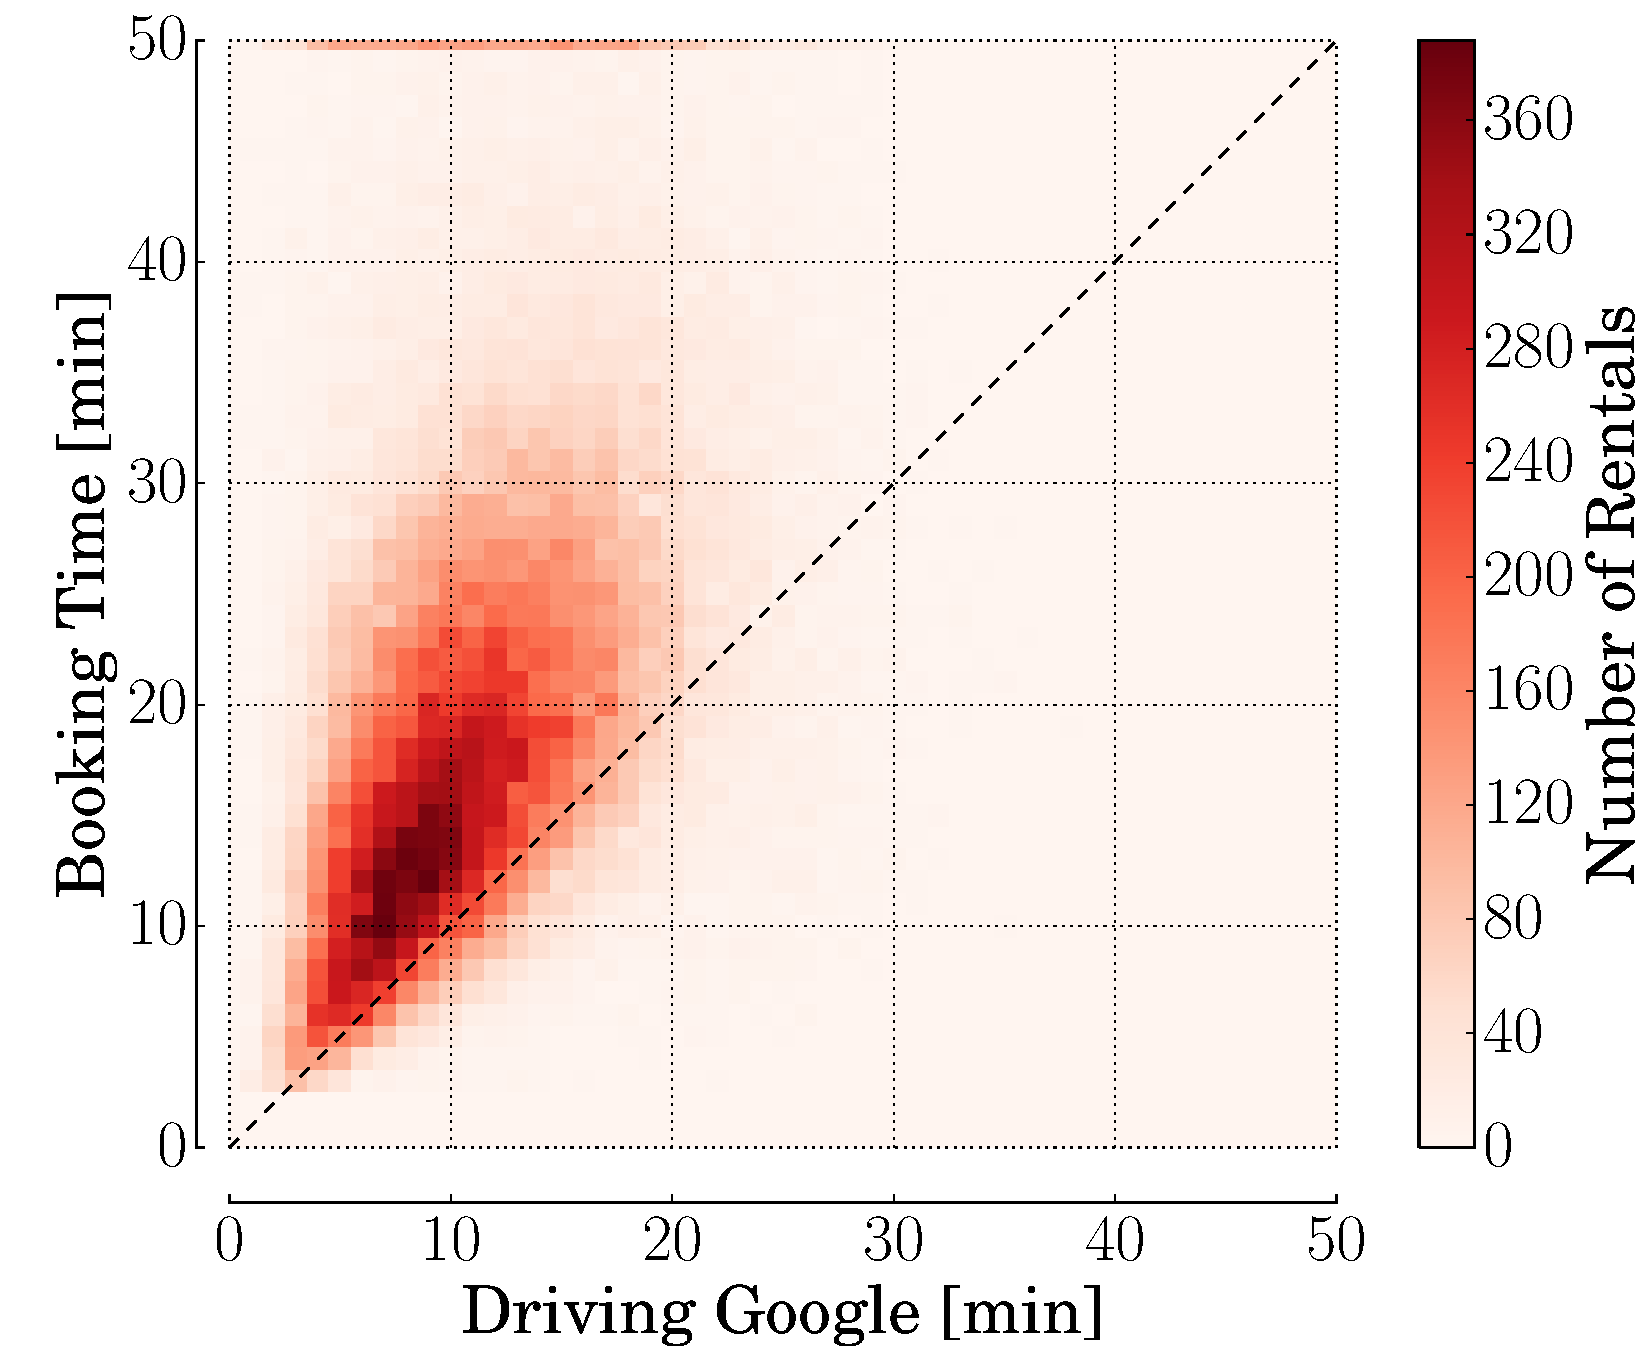
\includegraphics[width=0.5\columnwidth]{figures/car2go_faster_driving.pdf}}
%\subfloat[][ECDF of the difference between the expected driving time and the actual driving time]{\label{fig:cdf_faster_google}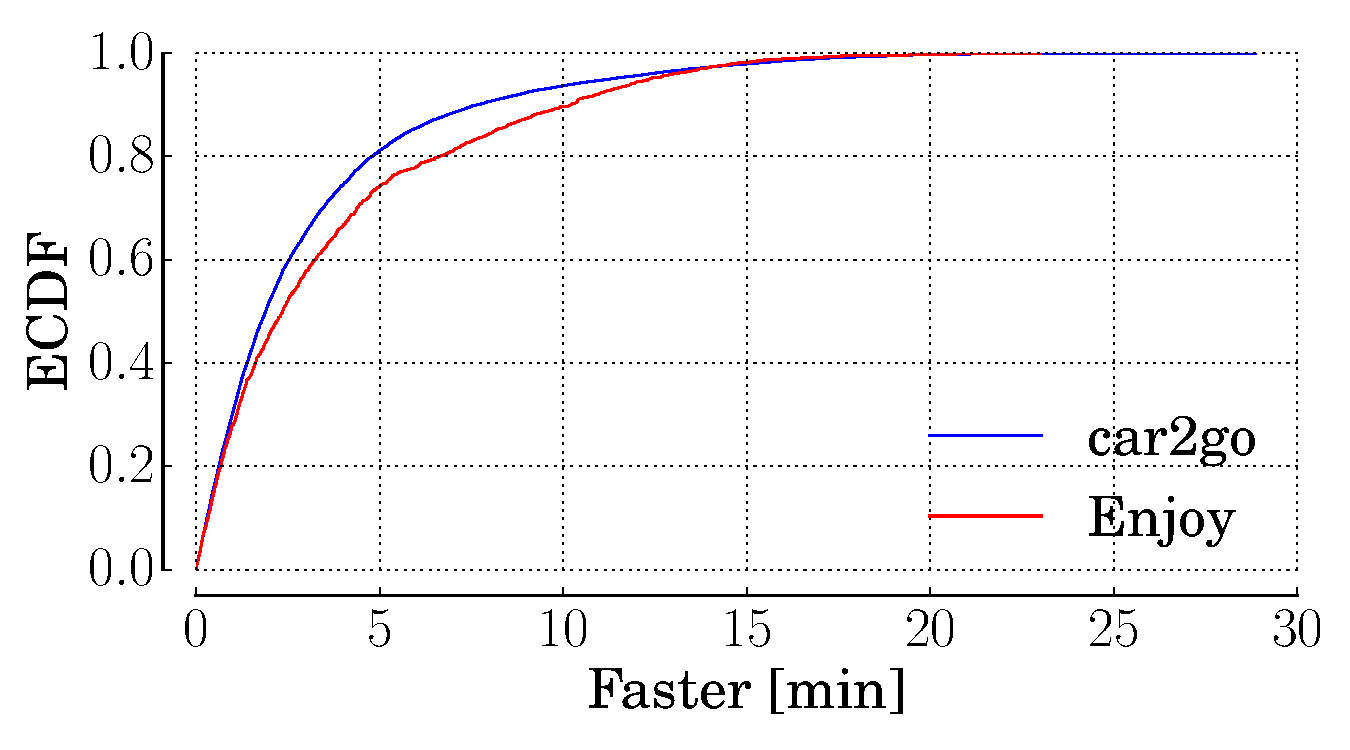
\includegraphics[width=0.5\columnwidth]{figures/faster_driving.pdf}}
%\caption{Users' driving habits}
%\end{figure}


At last, I leverage Google Directions APIs to extract public transport travel information for each vehicle's trip. I want to analyse another way of mobility in the urban area, and compare car sharing usage with respect to public transport. Results are shown in Figure~\ref{fig:3_5_public_transport}.
%The public transport duration includes both the time of travel and time of wait.
As one could expect, the majority of trips last less than public transport. The higher density is for bookings that last between 10 and 20 minutes. For longer trips, the discrepancy in terms of duration is higher, probably due to the longer path and the higher number of stops of the public transport. Conversely, I can interpret the points where the booking time is greater than  the public transport duration as trips where the customers spent a lot of time in reaching the car or finding a parking spot for the drop-off.

\begin{figure}[h!]
	\centering
	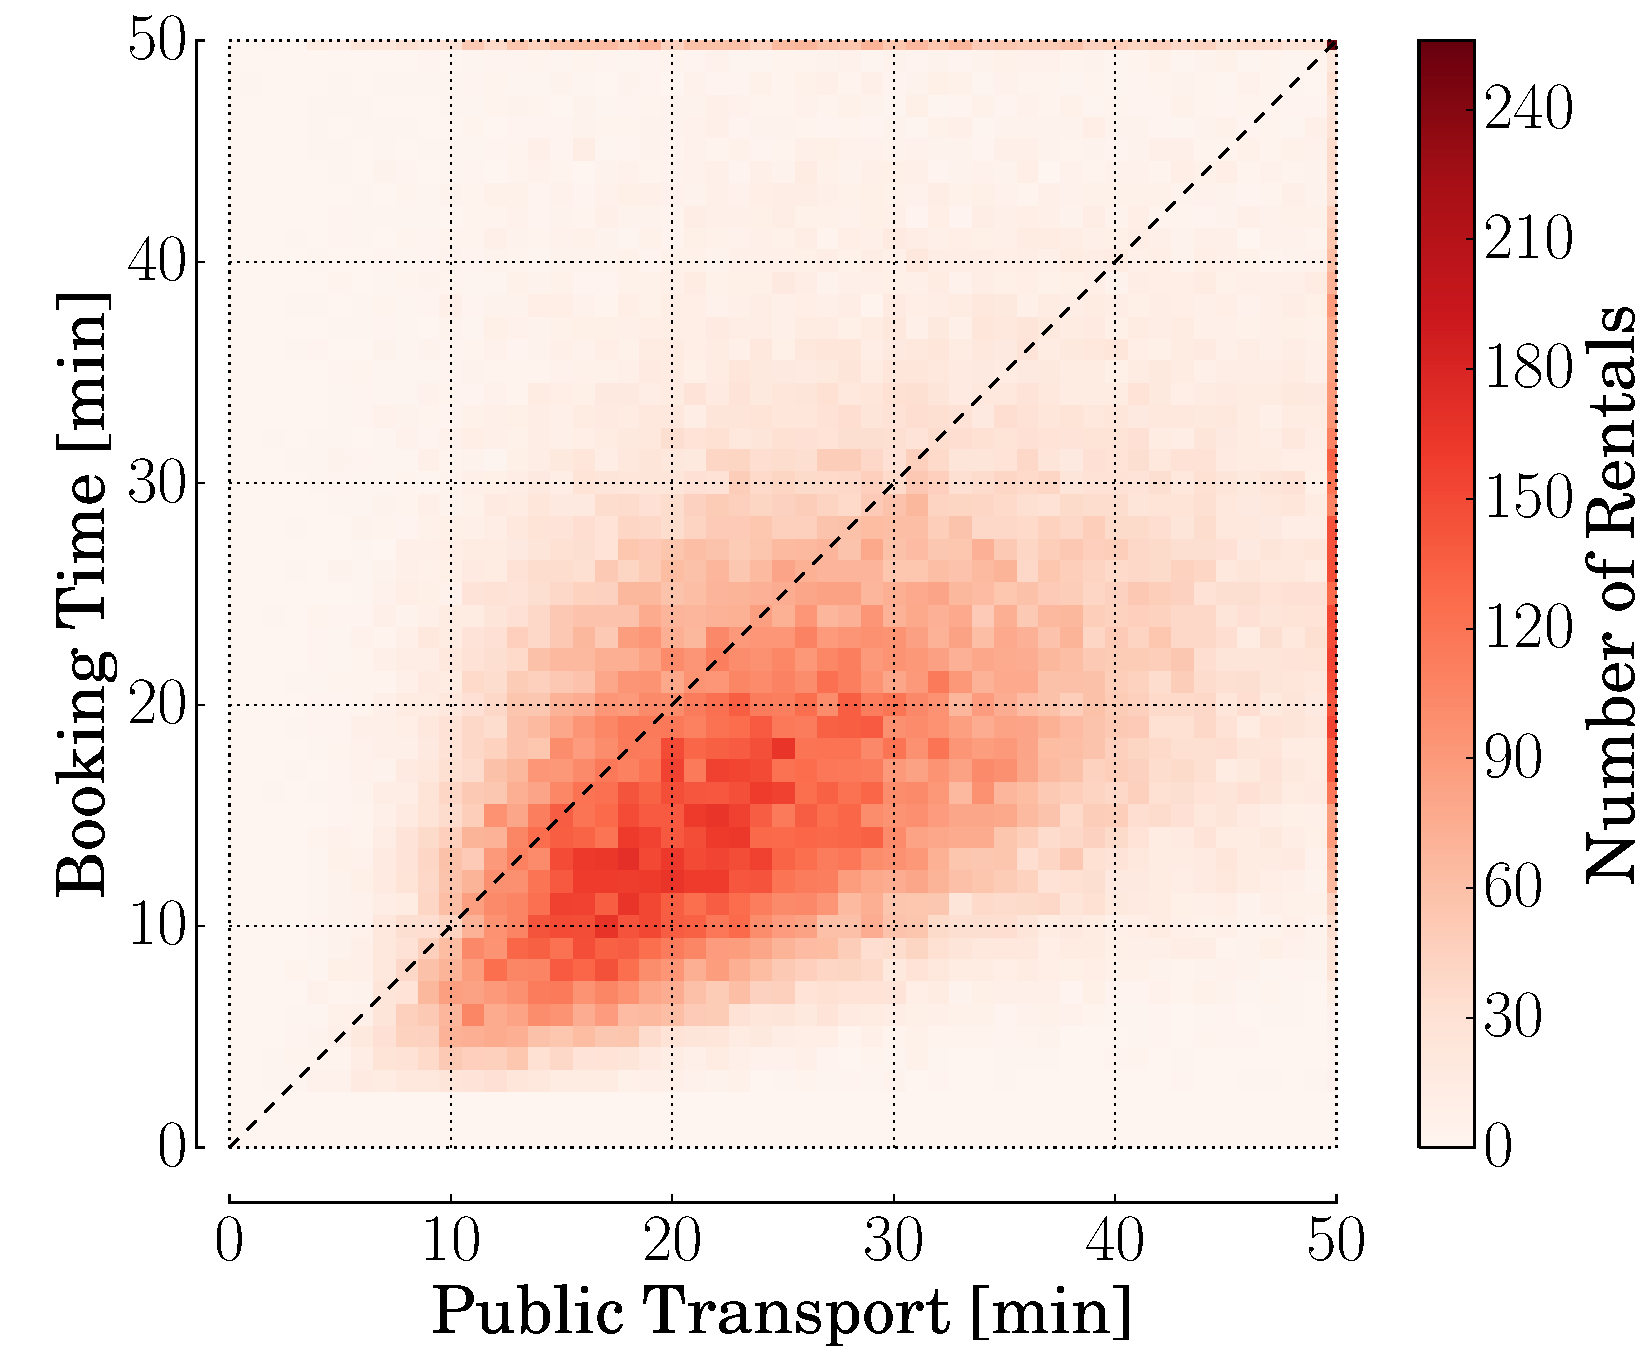
\includegraphics[width=0.85\columnwidth]{figures/car2go_faster_public.pdf}
	\caption{heatmap of the booking time  vs the estimated public transport time by Google\label{fig:3_5_public_transport}}
\end{figure}

To help to visualize the juxtaposition of car sharing and public transport, we extract from the data the probability of booking a car, conditioned to the public transport travel time. Figure~\ref{fig:pdf_transport}, reports on the X axis the public transport duration (as predicted by Google) in intervals of 5 minutes, and on the Y axis the probability of booking a car for each interval.
The distribution of probability is similar for both car2go and Enjoy. Higher values are reported for trips that can be covered by public transport between 15 and 35 minutes. Interestingly, car sharing mobility is not preferred for very short trips, while the distribution shows a significant tail for duration greater than 30 minutes. This behavior can be justified by the significant amount of time that can be saved with cars haring with respect to public transport.

\begin{figure}[h!]
	\centering
	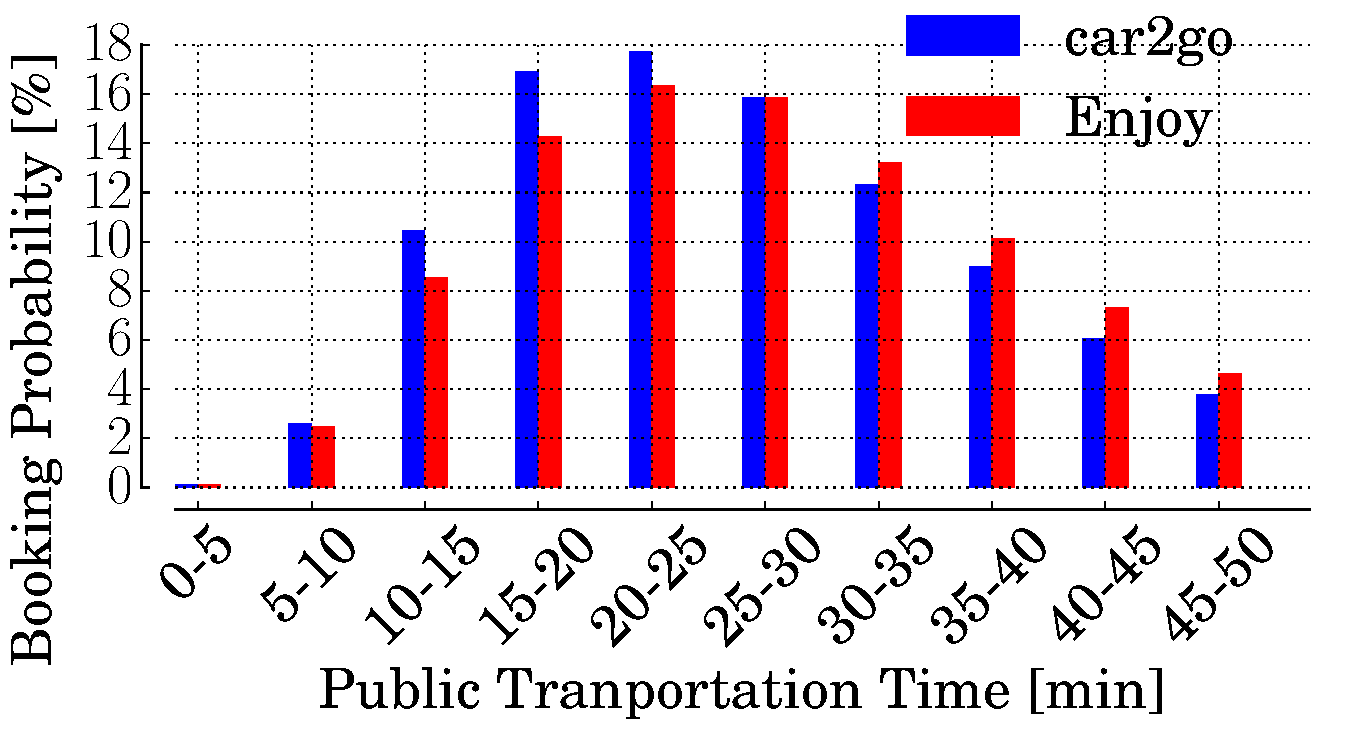
\includegraphics[width=0.85\columnwidth]{figures/public_tranport_probability.pdf}
	\caption{Public transportation vs car sharing\label{fig:3_5_public_tranport_probabilityt}}
\end{figure}
  
%  \begin{figure}[t!]
%  \centering     %%% not \center
%  \subfloat[][heatmap of the booking time  vs the estimated public tranport time by Google]{\label{fig:heatmap_transport}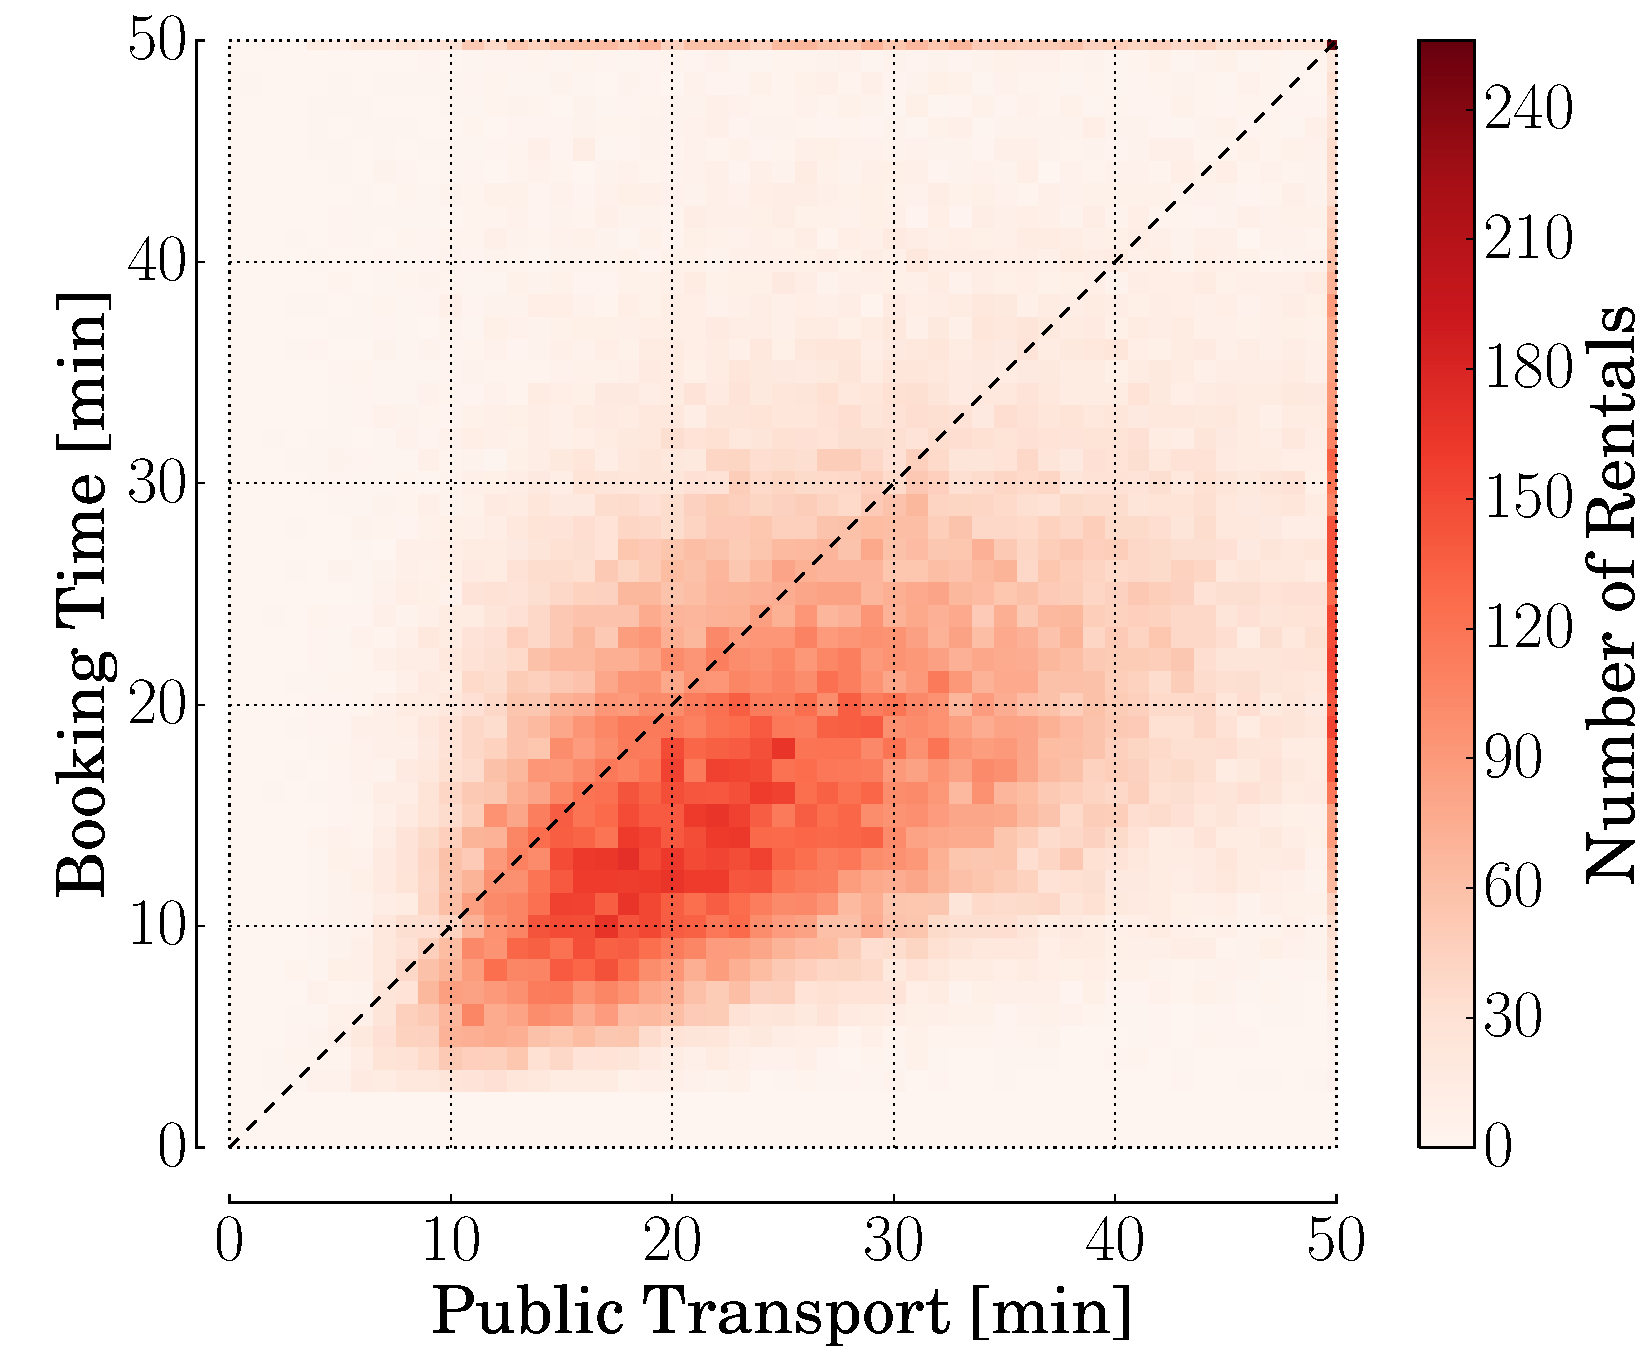
\includegraphics[width=0.5\columnwidth]{figures/car2go_faster_public.pdf}}
%  \subfloat[][Probability of using car sharing based on public transport time by Google]{\label{fig:pdf_transport}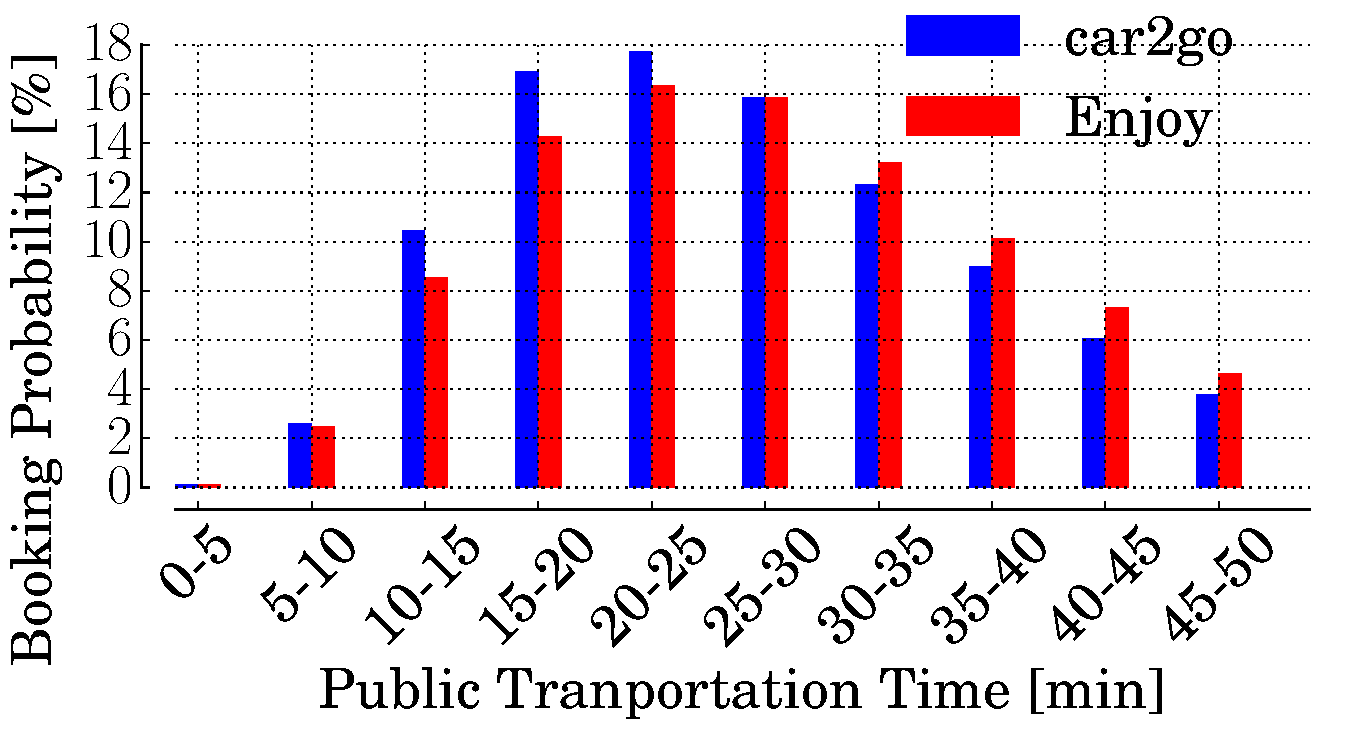
\includegraphics[width=0.5\columnwidth]{figures/public_tranport_probability.pdf}}
%  \caption{Public transportation vs car sharing \label{fig:public_transport}}
%  \end{figure}
%  
  
 
Finally, to globally understand how users tend to use the different services we report in Figure~\ref{fig:avg_comparison} the average time for: the Enjoy rentals (red curve), the car2go bookings (blue curve), the driving time (green curve), and public transport time (orange curve). To compute this value, for each hour we take all the rentals of interest, and then we compute the average value and report it. A first interesting aspect is that the average time of Enjoy is always greater then the car2go ones and for the pure driving time. Secondly, both show a similar trend with, a decreasing average duration during the night. As a consequence, it is unjustifiable ascribe this trend with traffic jam, instead, but more likely with an increase time in the reservation time and in the parking time. Finally, it is possible to appreciate how during the night the public transport takes more than 1 hour for trips which last less then 20 minutes by car. Instead, during the daytime the average public transport time get close to the car sharing time. 
%This demonstrates the goodness of the public transport system.



\begin{figure}[h!]
\centering
 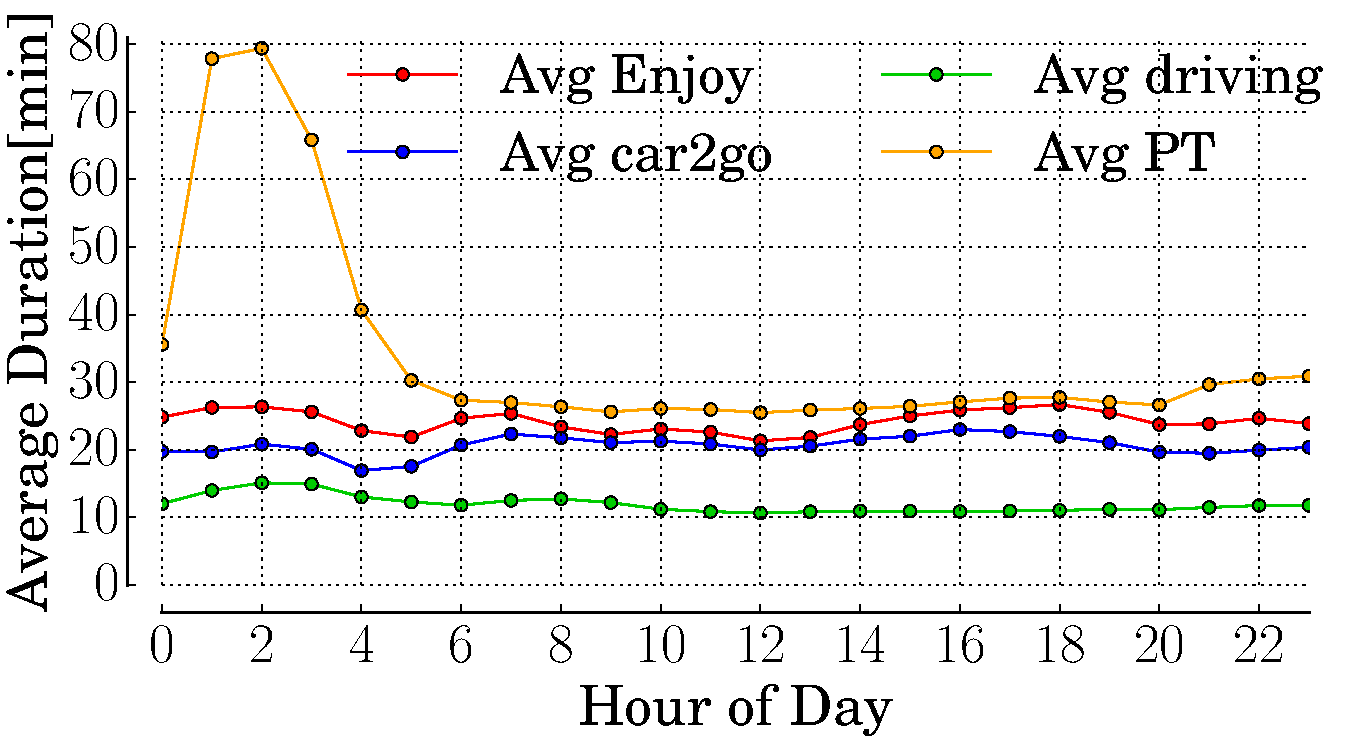
\includegraphics[width=0.85\columnwidth]{figures/average_duration.pdf}
 \caption{Average Time per transport solution per hour \label{fig:avg_comparison}}
\end{figure}

